\newpage
\section{PCB}
\subsection{First PCB Version}
The First PCB Version was a desaster. The PCBs arrived very fast, but the QFN Package had the wrong size.
ATMEL only produces QFN32 in 7x7mm. Therefore the design of the PCB hat to be changed to the smaller package,
but that gave me the Chance to shrink the Design to a smaller form factor.
The part which keeps the PCB from getting smaller is the Coin Cell Battery (CR2032).
On the PCBs there was the order number printed on the Front side, which would be visble in the final assembly.
\subsection{Second PCB Version}

The second PCB Version was designed from scratch. But the Front was the side with the Battery, so hopefully the Order Number would not be printed on the visible side of the PCB. This worked out very well for the second Version of the PCBs.
\subsection{PCB1}

since the PCBs finally arrived. it was possible to assemble all the parts.
The first PCB was assembled with some Cables soldered to the Testpins on the Backside of the Board.
And the Battery case was also not assembled.
Here is a Picture of the uncleaned but already soldered PCB
\begin{center}
  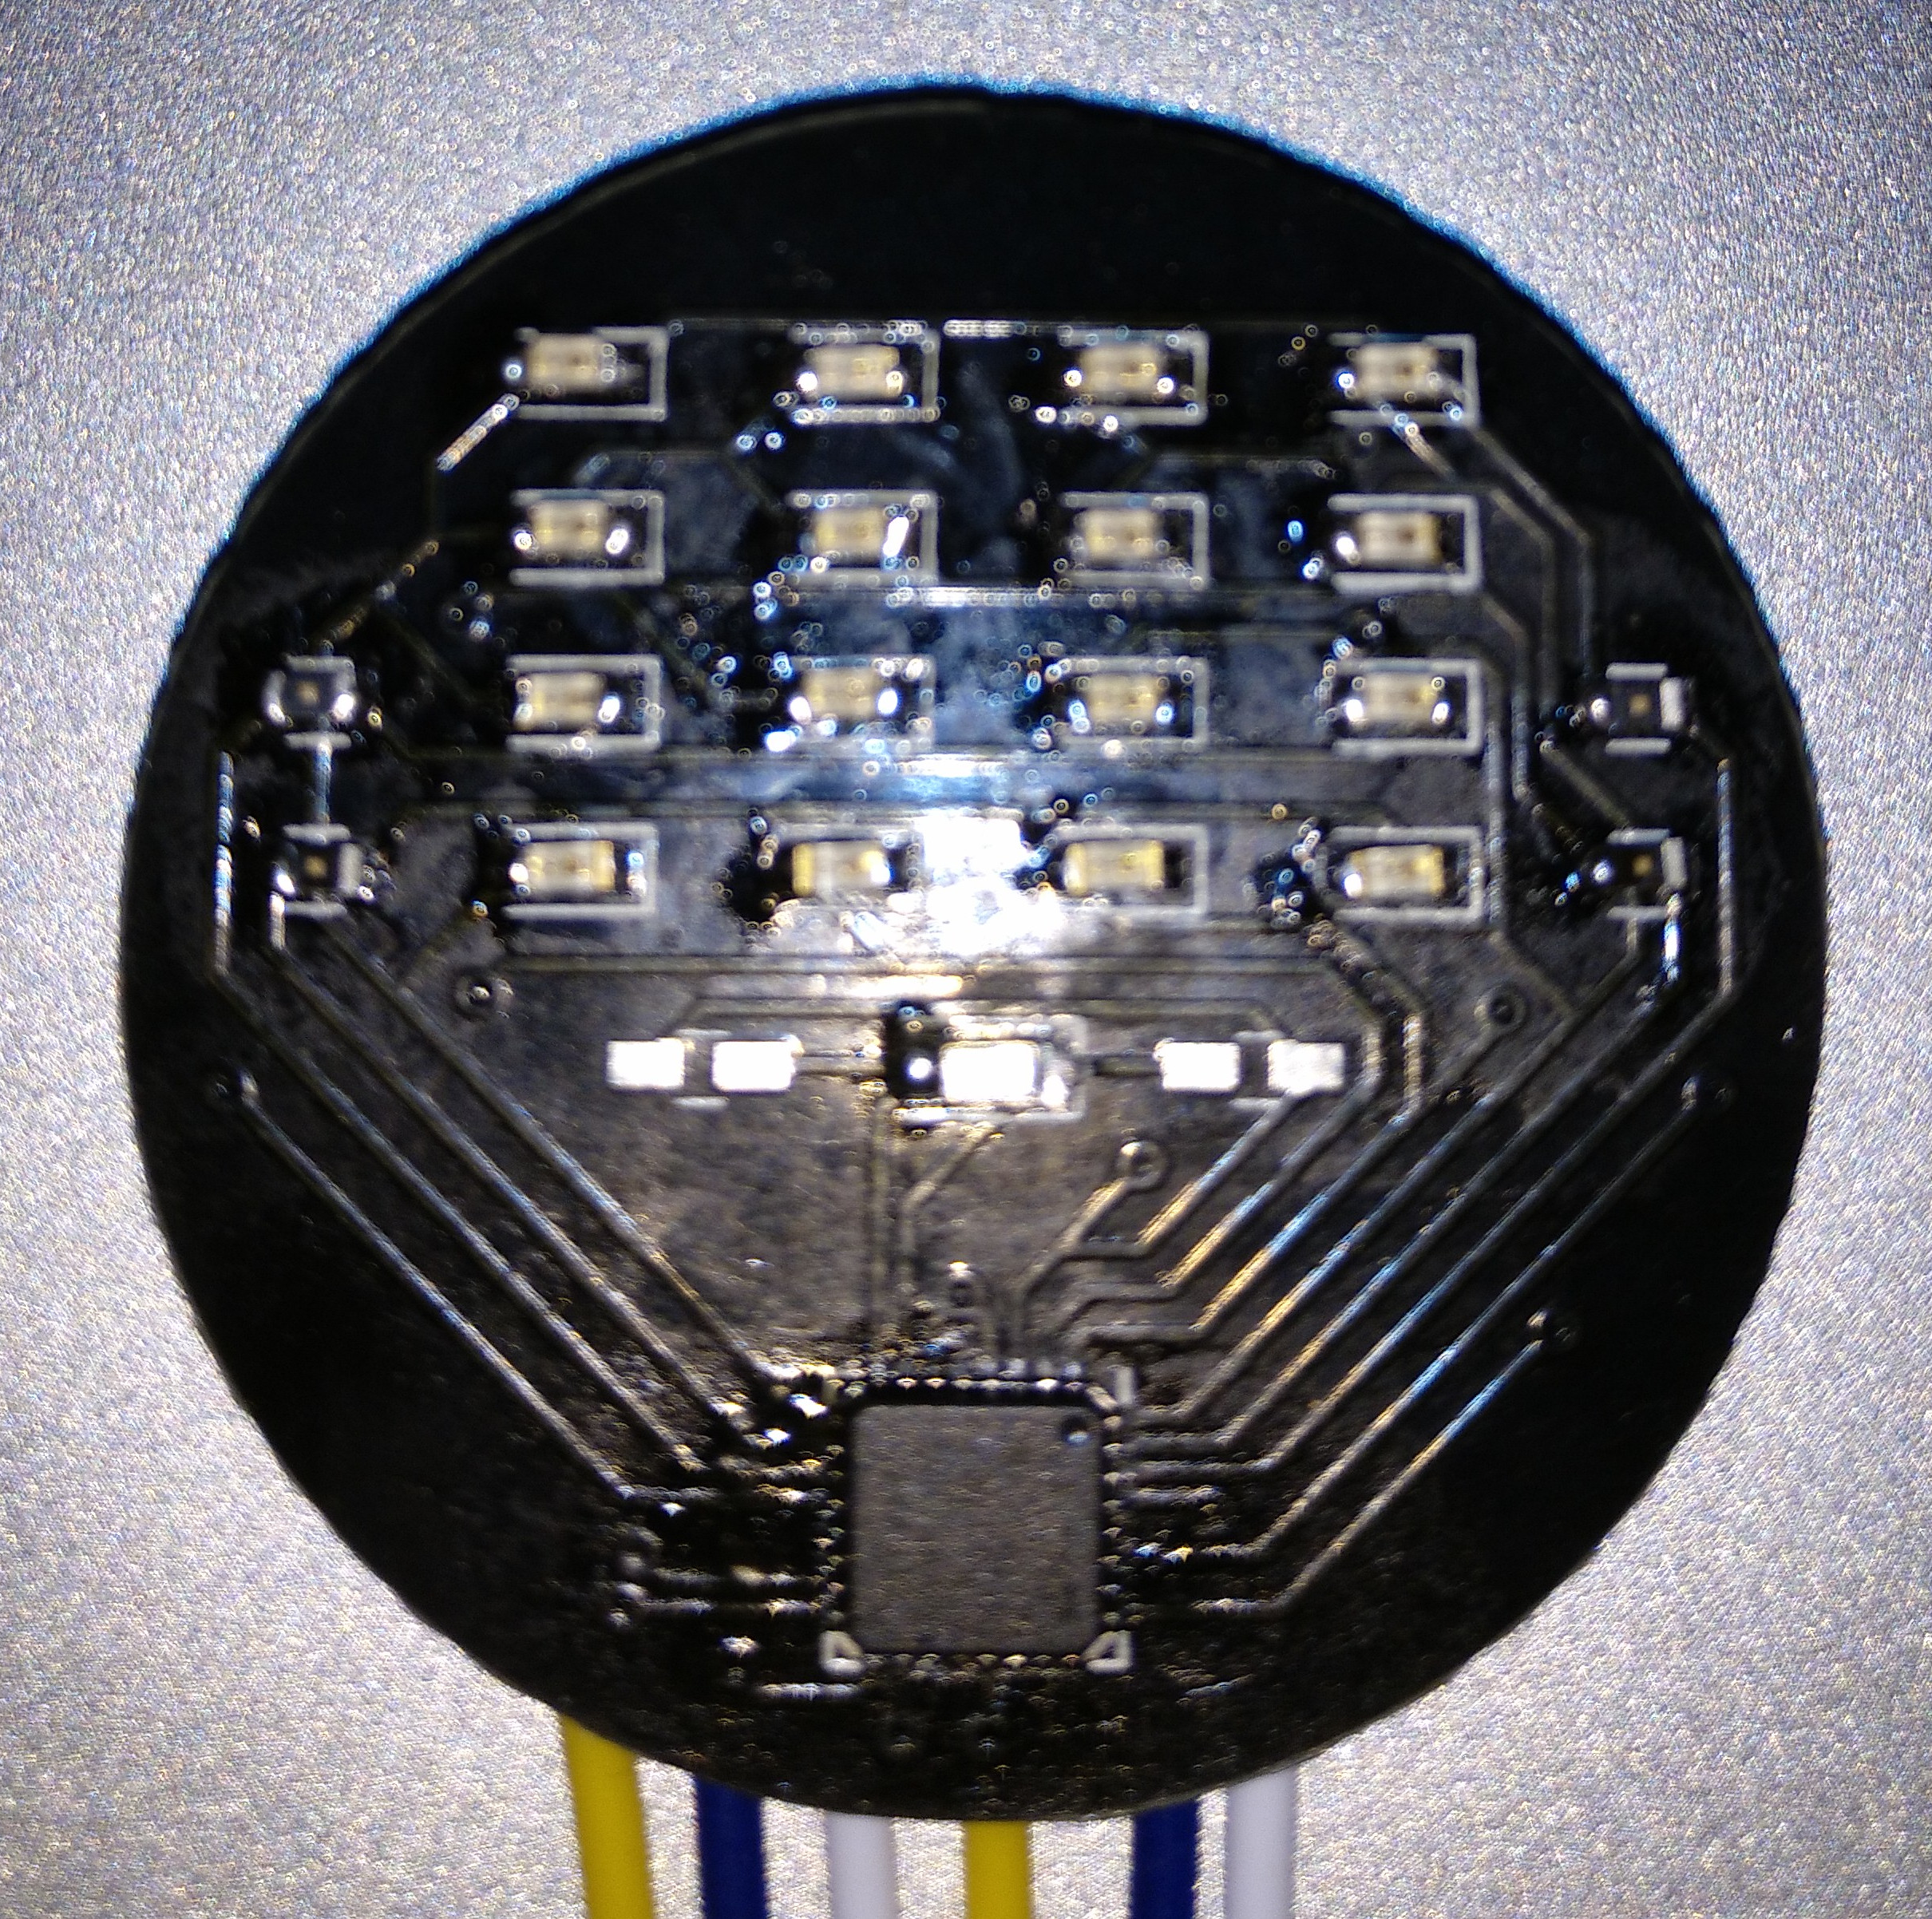
\includegraphics[width=0.5\textwidth]{../Pictures/PCB1_F1.jpg}
\end{center}

\subsection{PCB2}
The PCB2 was assembled and cleaned as a First Prototype with the Housing.\
Here aretwo Pictures of the PCB one without the LEDs turned on and one with the LEDs turned on.\
Brightness was set in the Program to 100/255 (see software void showLEDs, constant perc=100) 
\begin{center}
\includegraphics[width=0.45\textwidth]{../Pictures/PCB2_F1_off.jpg} \includegraphics[width=0.45\textwidth]{../Pictures/PCB2_F1_on.jpg}

\end{center}

\subsection{PCB3}
The third PCB was ordered at [aisler.net](https://aisler.net). It only took around one and a half week to arrive(to Germany).\
The PCB was not completely milled out. It was in a carrier PCB with rectangular shape, but it was easy to remove.\
I had to sand the edges a bit, since it was a bit rough on the parts where i removed the connections to the carrier, since i had to sand the PCB anyway to fit in the Housing that was no big problem.\
The overall Quality of the PCBs is very good, but you can not choose the thicknes or color of the PCB.\
\begin{center}
  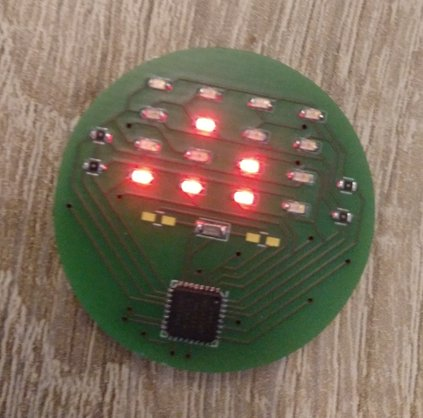
\includegraphics[width=0.5\textwidth]{../Pictures/PCB3.jpg}
\end{center}

\newpage
\section{PCB for an analog Version}
After the PCBs for the BCD Version were working, i also created an analog Version, so i dont have to explain the Clock everytime ;-)

The Analog Watch features the same Schematics for the basic clock functionality, but the display is done via Charlieplexing the LEDs. There are 4 Clustes with 4 Pins which drive all the 42 LEDs. 12 LEDs on the inner ring are displaying the hours. On the outer ring 30 LEDs display the Minutes. Since it was not possible to fit 60 LEDs on the outer ring, uneven numbers are shown while lighting up the two neighbouring LEDs.
\begin{center}
  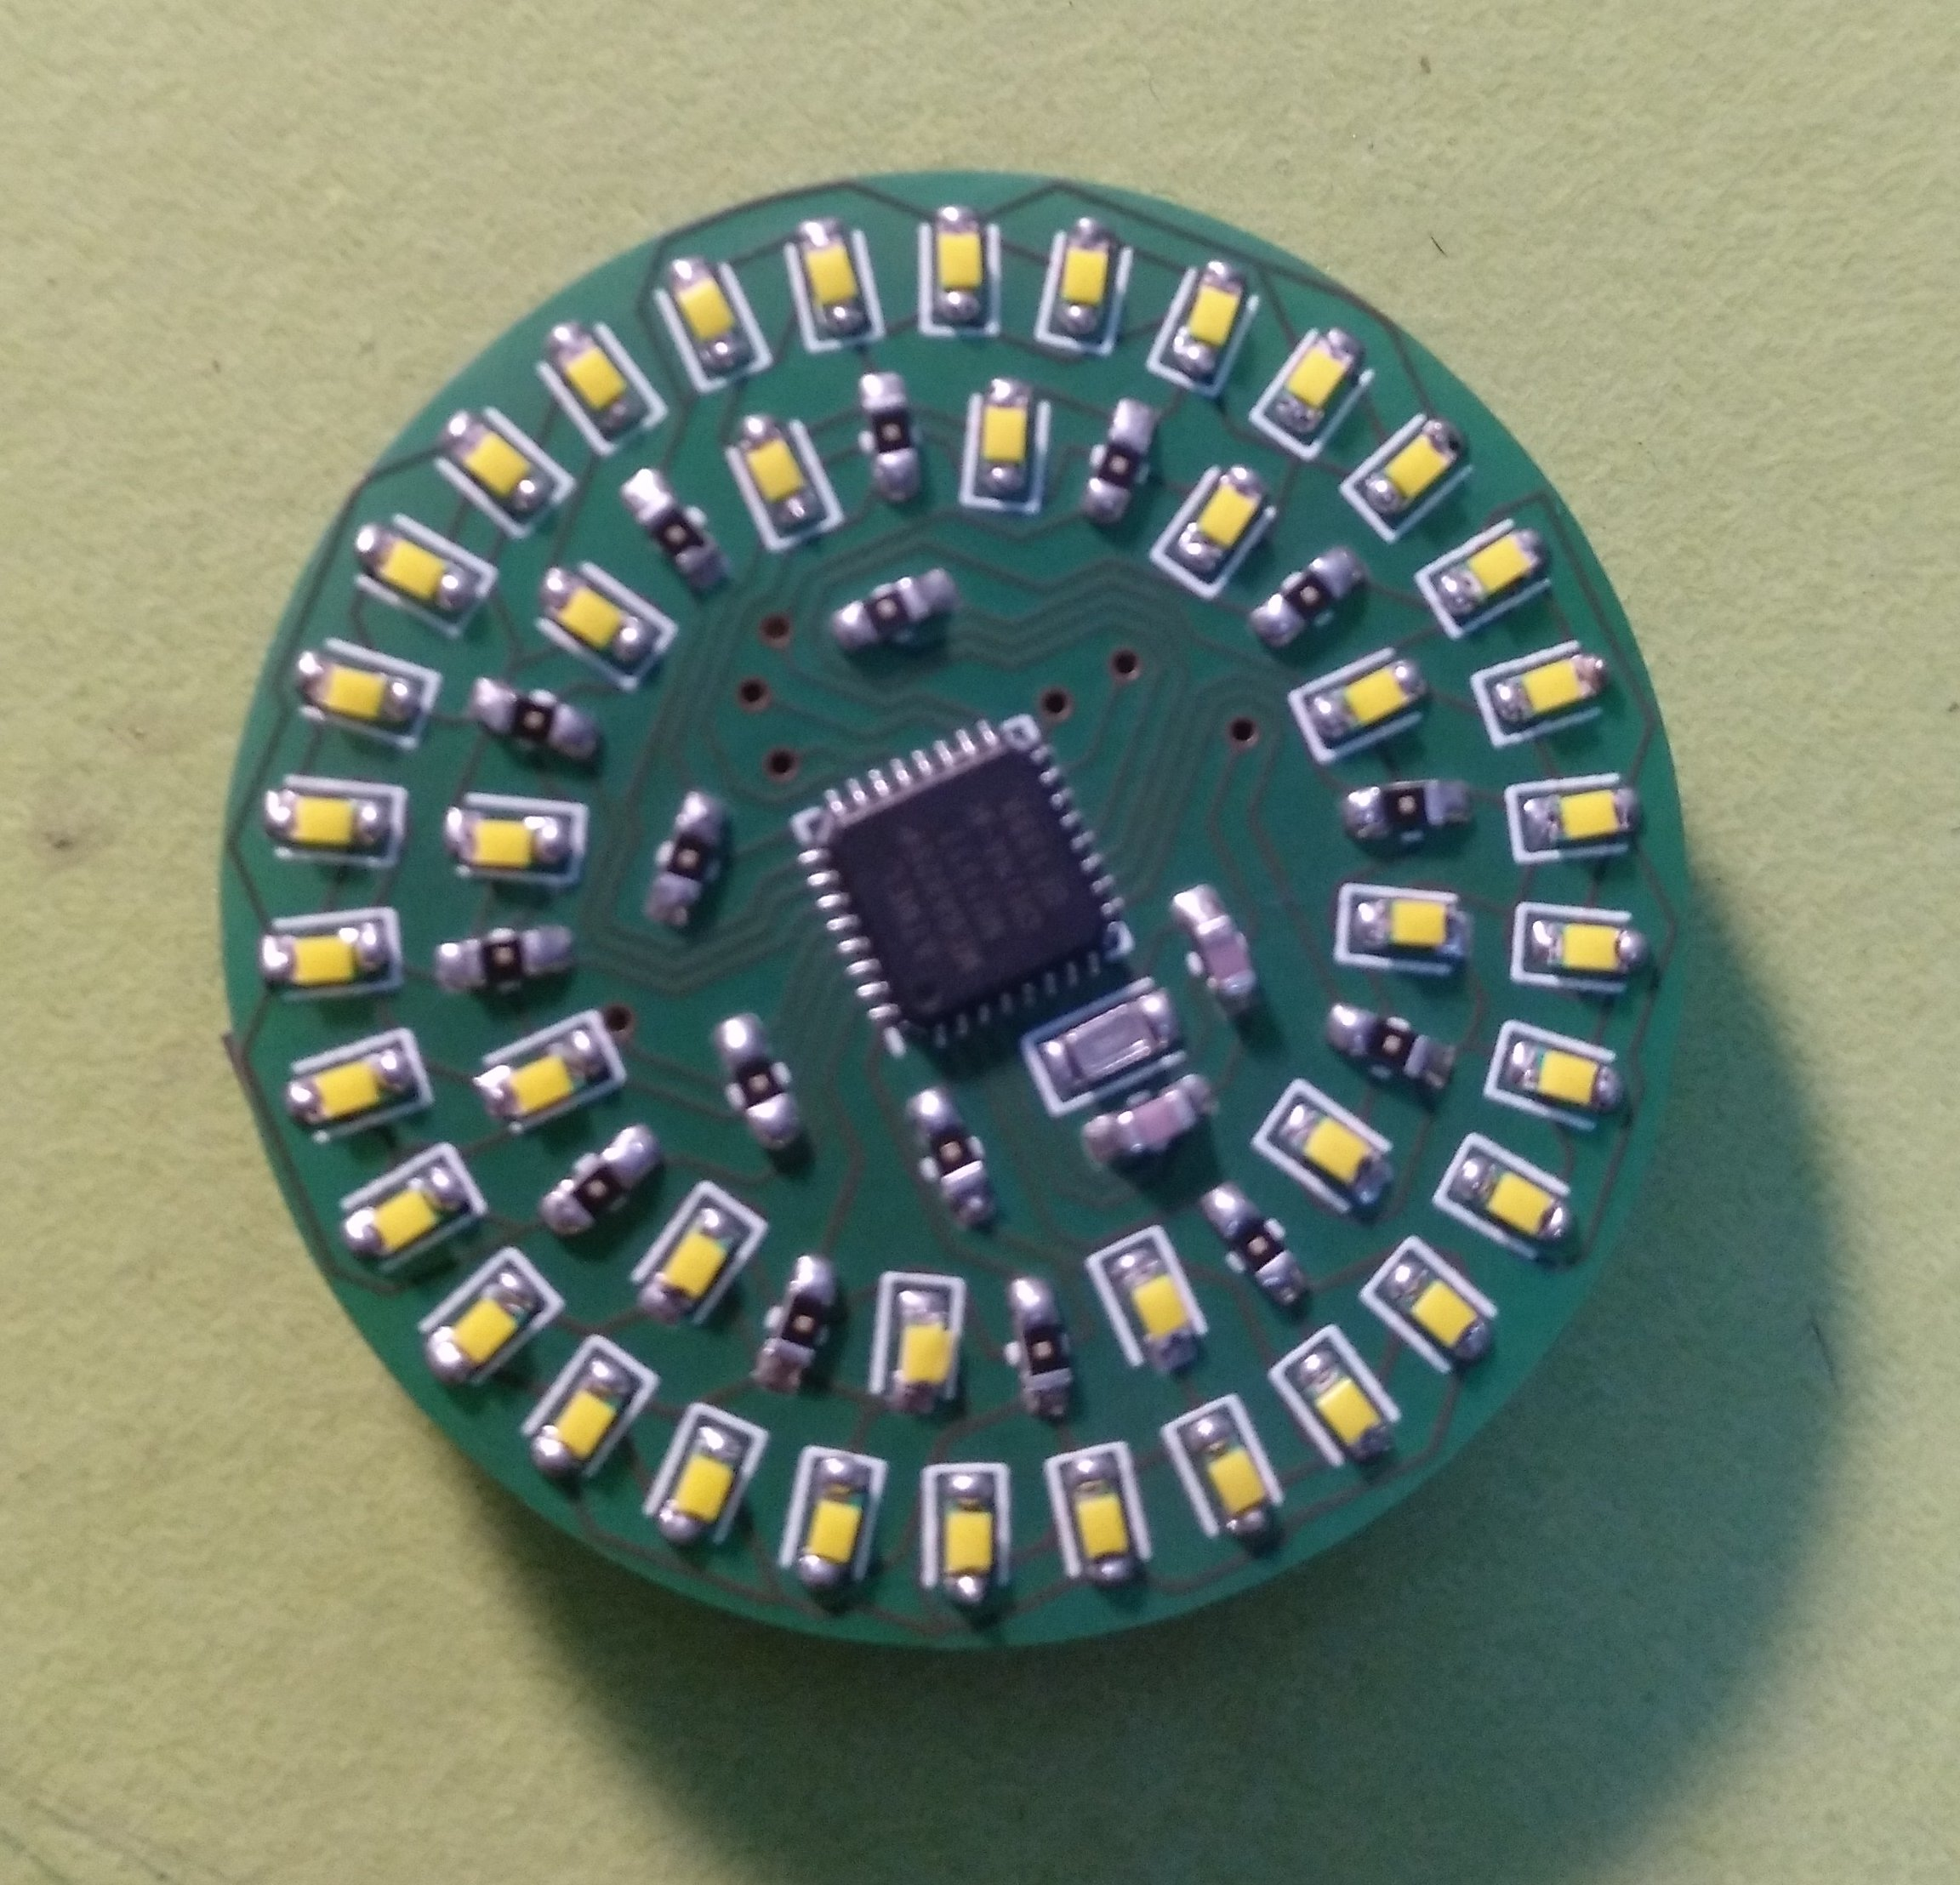
\includegraphics[width=0.5\textwidth]{../Pictures/AnalogPCB.jpg}
\end{center}
\newpage
\subsection{first Watch which i gave away}
The first Watch i gave away was one of the analog PCB ones i built for my dads birthday.
for this Watch i replaced all the resistors for the LEDs with Zero $\Omega$ resistors, so the LEDs got more bright and are clearly readable also in the sunlight.
\begin{center}
  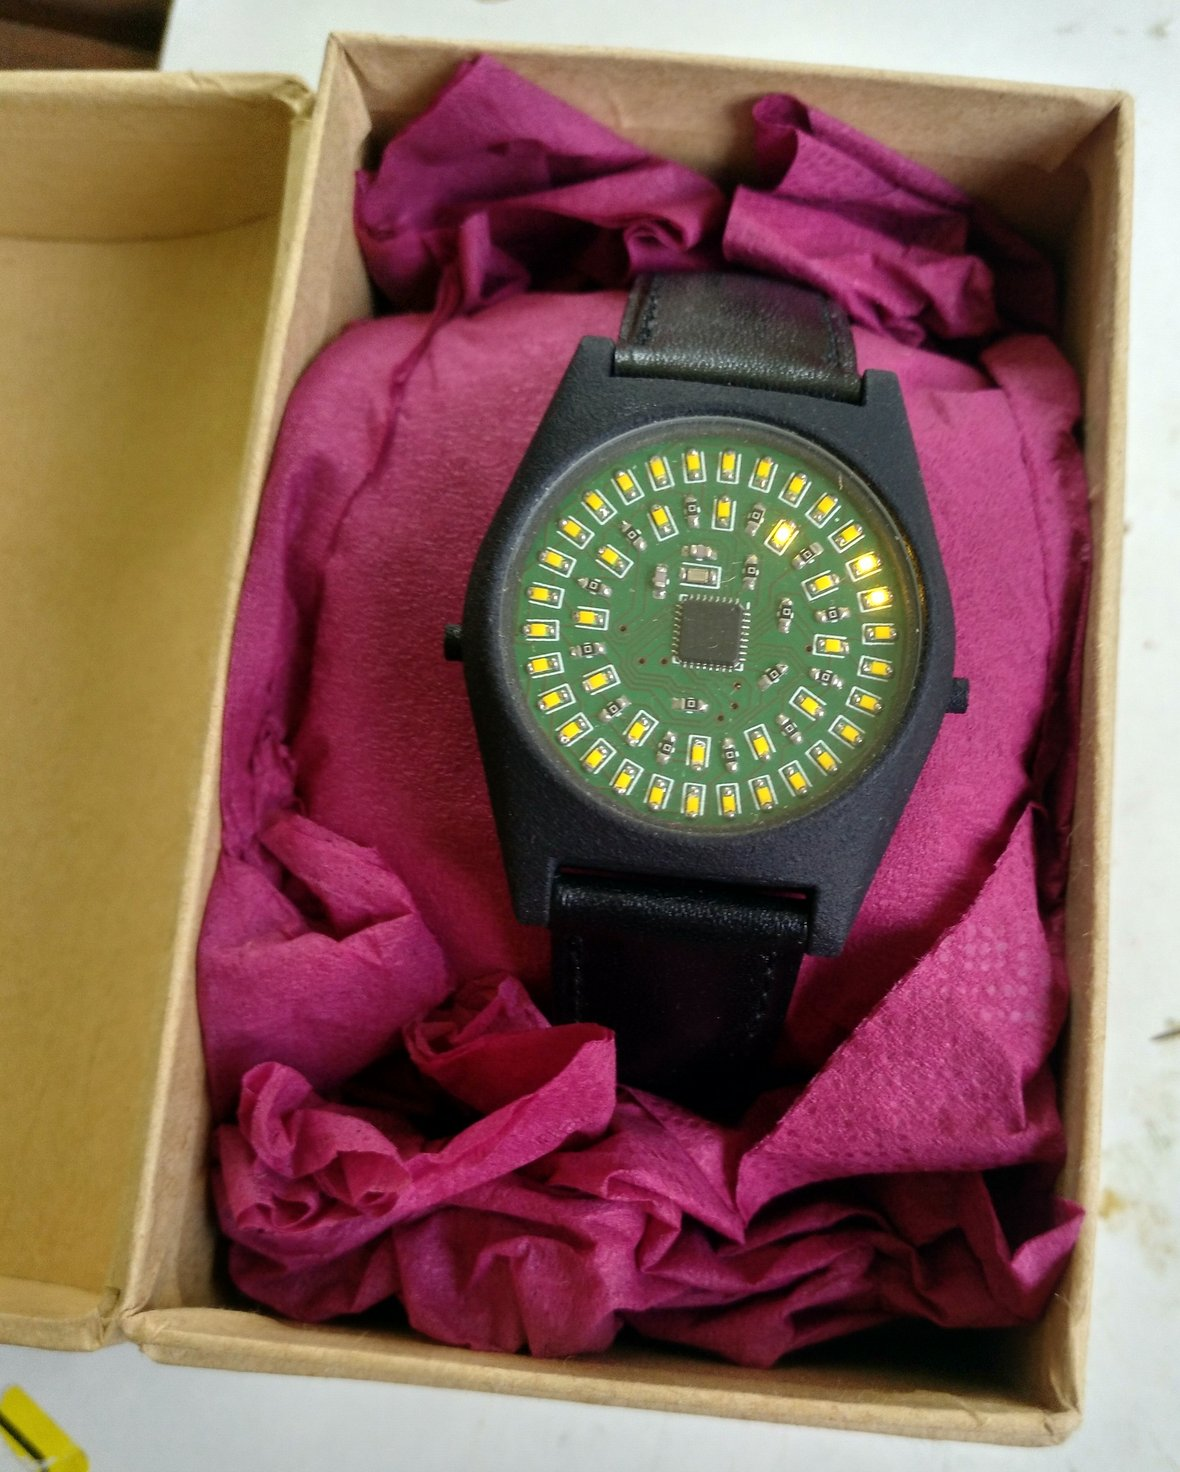
\includegraphics[width=0.7\textwidth]{../Pictures/AnalogWatch1.jpg}
\end{center}